\documentclass[journal]{IEEEtran}
\usepackage{cite}
\usepackage{amsmath,amssymb,amsfonts}
\usepackage{algorithmic}
\usepackage{graphicx}
\usepackage{textcomp}
\usepackage{wrapfig}
\usepackage{caption}
\usepackage{subcaption}
\usepackage{enumitem}
\usepackage[most]{tcolorbox}
\usepackage{listings}
\usepackage{xcolor}

\lstdefinelanguage{RISCV}{
  keywords={ld, sd, and, or, add, sub, beq, jal},
  keywordstyle=\color{blue}\bfseries,
  comment=[l]{\#},
  commentstyle=\color{green!50!black}\itshape,
  basicstyle=\small\ttfamily,
  breaklines=true,
}

\lstdefinelanguage{Verilog}{
  keywords={module, endmodule, input, output, wire, reg, always, begin, end, if, else, case, endcase, assign, posedge, negedge, clk, reset},
  keywordstyle=\color{blue}\bfseries,
  comment=[l]{//},
  morecomment=[s]{/*}{*/},
  commentstyle=\color{green!50!black}\itshape,
  string=[b]",
  stringstyle=\color{red},
  basicstyle=\small\ttfamily,
  breaklines=true,
  breakatwhitespace=true,
  breakindent=0pt,
  showstringspaces=false,
}

\ifCLASSINFOpdf
\else
\fi

\hyphenation{op-tical net-works semi-conduc-tor}


\begin{document}
\title{IPA Project Report (Phase II) \\ Implementation of a 64-bit RISC-V CPU}
\author{
    \begin{tabular}[t]{c@{\extracolsep{8em}}c@{\extracolsep{8em}}c}
        Ritvik Avula        & Pavani Malchuru     & Nikhilesh Nallavelli \\
        Roll No: 2024112019 & Roll No: 2024102043 & Roll No: 2024102051  \\
    \end{tabular}
}

% The paper headers
\markboth{IPA Project Report}{RV64I CPU}

\maketitle

\begin{abstract}
    This report presents the next phase in the design and implementation of a
    64-bit RISC-V CPU using Verilog. In this report, we provide a comprehensive
    overview of the pipelined architecture and detail the different kinds of
    hazard handling mechanisms that were implemented in the project.
\end{abstract}


\section{Introduction and Background}

\IEEEPARstart{T}{he} RISC-V ISA is an open source instruction set architecture
that focuses on maintaining simple hardware and using basic instructions in
order to design and program more complicated entities. This simplicity makes
RISC-V an ideal choice for custom processor design. The instruction set is
modular, allowing implementations to support only the necessary base
instructions (RV64I) or extend with optional extensions for floating-point
operations, atomic instructions, and more. In this project, we focus on
implementing the RV64I base integer instruction set for 64-bit systems.

Of all the instructions in the base RV64I ISA, we've implemented the following
subset of instructions:

\begin{itemize}
    \item \textbf{R-type} (add, add/or/xor, sll/srl/sra)
    \item \textbf{I-type} (addi and etc..., ld, jalr)
    \item \textbf{S-type} (sd)
    \item \textbf{B-type} (beq)
    \item \textbf{J-type} (jal)
\end{itemize}

\section{Overview of the Pipelined Architecture}

\begin{figure}[!ht]
    \centering
    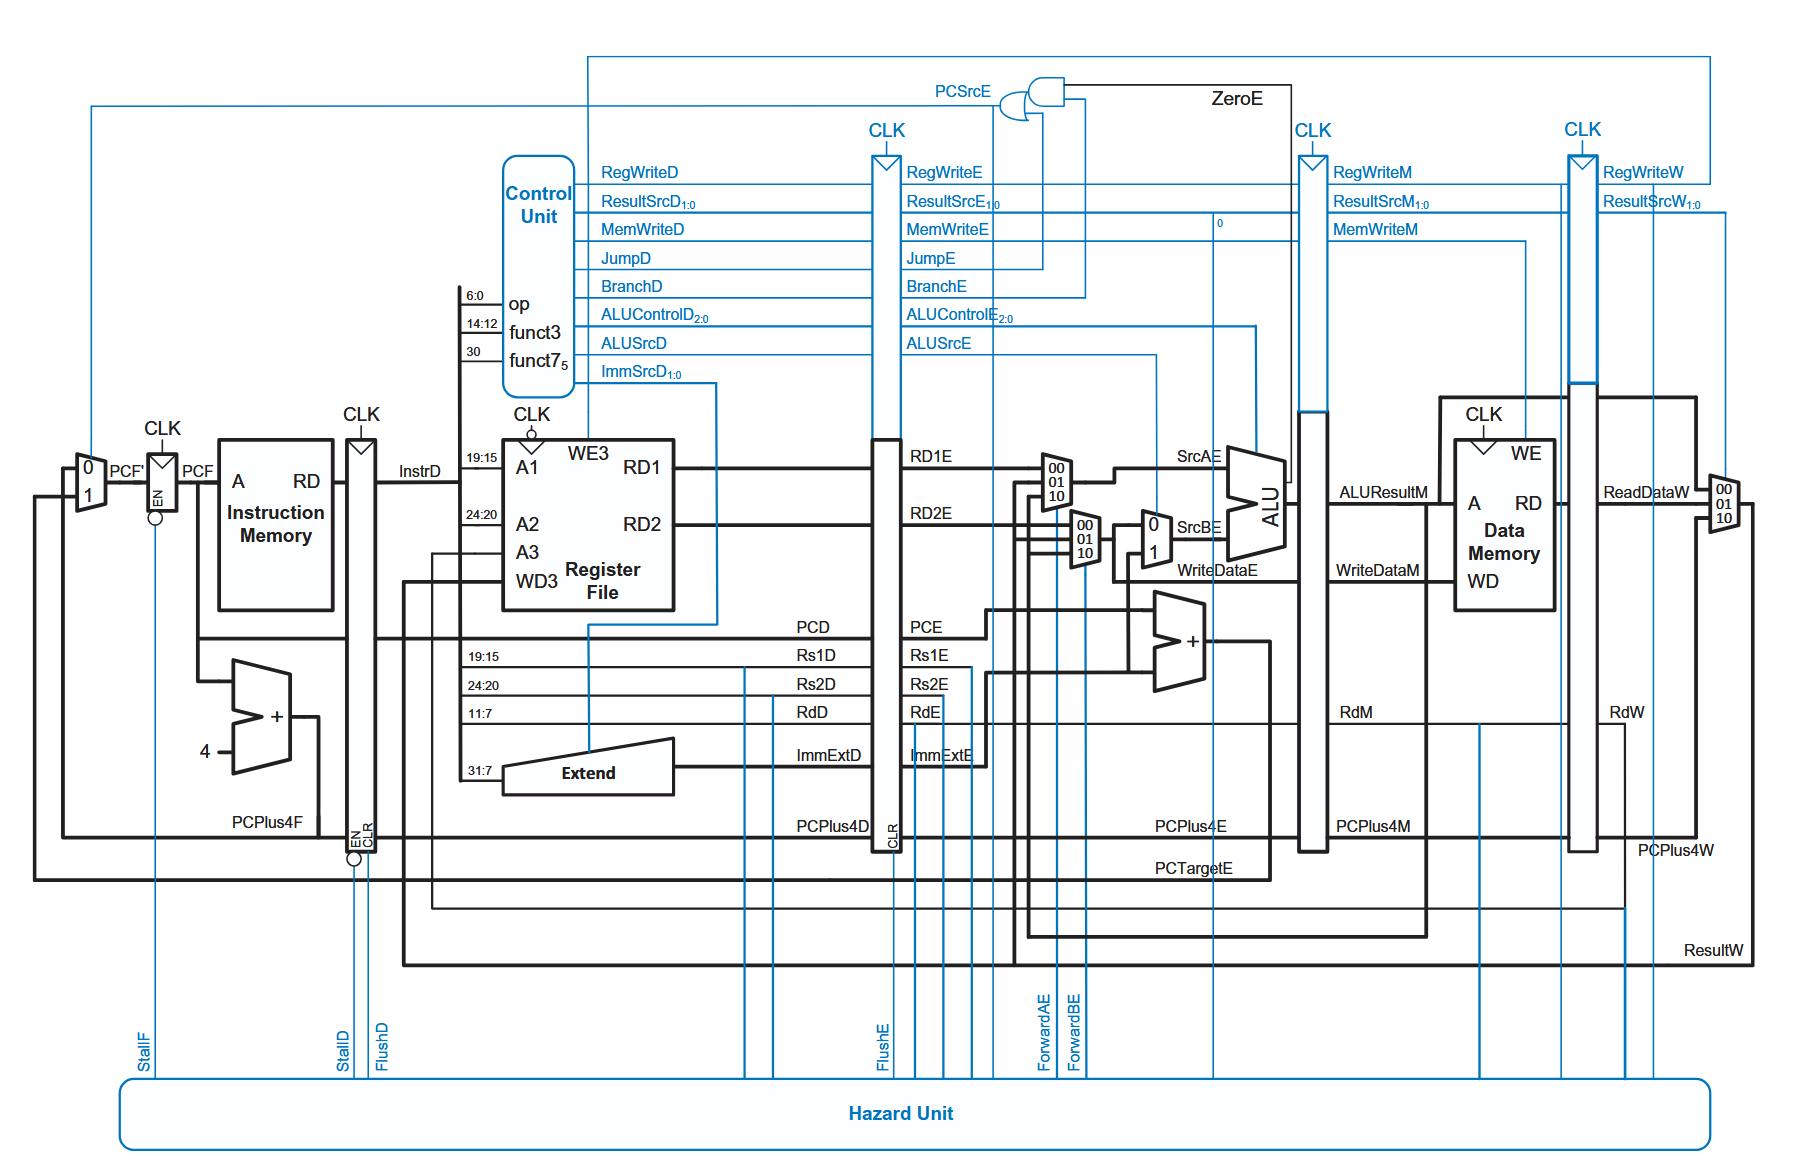
\includegraphics[width=0.45\textwidth]{figures/pipelined_processor.png}
    \caption{High-level architecture of the RV64I pipelined processor. Courtesy of \textit{Digital Design and Computer Architecture,}
        \cite{harris2021digital}}
    \label{fig:pipelined_processor}
\end{figure}

The RV64I CPU consists of several key modules that work in conjunction to
execute instructions. Fig. \ref{fig:pipelined_processor} illustrates the high-level
architecture of the processor.

The datapath consists of the following main components:

\begin{enumerate}
    \item \textbf{Program Counter (PC):} Stores the address of the current
          instruction and increments to fetch the next instruction
    \item \textbf{Instruction Memory:} Stores the program instructions
    \item \textbf{Register File:} Contains 32 general-purpose 64-bit registers
    \item \textbf{Arithmetic Logic Unit (ALU):} Performs computations - either
          arithmetic or to declare flags to be used in conditional operations
    \item \textbf{Control Unit:} Decodes and instruction and generates control
          signals that determine which modules should be active during the
          instruction cycle
    \item \textbf{Immediate Generator:} Extracts and extends immediate values from
          instructions
\end{enumerate}

In this part of the project, we've added a \textbf{Hazard Detection Unit} to
account for various hazards that pop up when pipelining a processor - namely
hazards like:

\begin{enumerate}
    \item \textbf{Data Hazards:} Resolves most RAW data hazards by introducing
          forwarding paths from MEM and WB stages to the EX stage inputs.
    \item \textbf{Control Hazards:} Detects branch control hazards and flushes
          the buffers between stages if needed.
\end{enumerate}

\section{Solving Hazards}

This section goes into more detail about how different types of hazards are
solved in the pipelined CPU.

\subsection{Data Hazards}
Data hazards occur when an instruction depends on the result of a previous
instruction that has not yet completed executing. In a pipelined processor,
multiple instructions are in different stages simultaneously - which can lead to
situations where data is read before it has been written.

In our version of a pipelined CPU, we majorly try to solve
\textbf{Read-After-Write (RAW) Hazards} - In this type of data hazard, an
instruction tries to read a register before a previous instruction writes to it.

\subsubsection{\textbf{RAW Hazards and Forwarding}}
The textbook \textit{Computer Organization And Design}
\cite{patterson2022computer} describes two major pairs of RAW hazards:

\begin{itemize}
    \item[1a.] EX/MEM.RegisterRd = ID/EX.RegisterRs1
    \item[1b.] EX/MEM.RegisterRd = ID/EX.RegisterRs2
    \item[2a.] MEM/WB.RegisterRd = ID/EX.RegisterRs1
    \item[2b.] MEM/WB.RegisterRd = ID/EX.RegisterRs2
\end{itemize}
Consider the following instruction sequence:

\begin{verbatim}
    add x5, x1, x2    # x5 = x1 + x2
    sub x6, x5, x3    # x6 = x5 - x3 
\end{verbatim}

Without hazard handling, when \texttt{sub} reaches the EX stage and
attempts to read \texttt{x5}, the \texttt{add} instruction may still be in the
MEM or WB stage, meaning the updated value of \texttt{x5} has not yet
been written back to the register file.

We can fix these problems by \textbf{forwarding the data}. The forwarding
unit compares the source registers of the instruction in the EX stage
(\texttt{rs1\_E}, \texttt{rs2\_E}) against destination registers in later stages
(\texttt{rd\_M} in MEM stage and \texttt{rd\_W} in WB stage). When a
match is detected and the corresponding RegWrite signal is enabled, the
forwarding unit selects the computed value directly from the later stage instead
of using the stale value from the register file.

Two forwarding select signals are generated:
\begin{itemize}
    \item \textbf{ForwardA:} Controls which value feeds ALU input A.
          \begin{itemize}
              \item \texttt{00}: Use register file output (no hazard)
              \item \texttt{01}: Forward from WB
              \item \texttt{10}: Forward from MEM
          \end{itemize}
    \item \textbf{ForwardB:} Controls which value feeds ALU input B. (same encoding)
\end{itemize}

Note that when comparing register addresses, both forwarding paths activity, we
give priority to the value in MEM rather than WB because it contains the more
recent result.

Hence, the code snippet looks like the following:

\begin{lstlisting}[language=verilog]
if(((rs1_e == rd_m) && reg_write_m) && 
   (rs1_e != 0)
  ) // EX-MEM hazard
       forward_ae = 2'b10;
   else if(((rs1_e == rd_w) && reg_write_w) && (rs1_e != 0)) // MEM-WB hazard
       forward_ae = 2'b01;
   else
       forward_ae = 2'b00;
\end{lstlisting}

Of course, the same follows for \texttt{rs2} and \texttt{forward\_be}.

\begin{tcolorbox}
    \textbf{A Note on Load-to-Store Forwarding}

    An important special case occurs when a load instruction is immediately
    followed by a store instruction that uses the loaded value:

    \begin{lstlisting}[language=RISCV]
ld x5, 0(x1)    # Load x5 from memory
sd x5, 8(x2)    # Store x5 to different address in memory
\end{lstlisting}

    In this scenario, the store instruction in the Memory stage needs the
    value from \texttt{x5} as its write data. Since the load result becomes
    available at the end of the Memory stage (or from the MEM/WB pipeline
    register), we implement a forwarding path that routes the loaded data
    directly to the store's write data input.

    This eliminates the need for the data to first pass through the Writeback stage and register file, allowing back-to-back load-store operations without stalling.
\end{tcolorbox}

This forwarding mechanism eliminates most RAW hazards without
stalling the pipeline.

\subsubsection{\textbf{Load-Use Hazards and Stalling}}

Forwarding cannot solve all RAW hazards. A critical exception is the
\textbf{load-use hazard}, where a load instruction is immediately followed by an
instruction that uses the loaded data:

\begin{verbatim}
    ld x5, 0(x1)      # Load x5 from memory
    add x6, x5, x2    # Immediately use x5
\end{verbatim}

The problem is that the data from memory becomes available only at the end of
the MEM stage, but the \texttt{add} instruction needs it at the beginning of
the EX stage—one cycle too early. Forwarding paths exist, but the data
simply isn't ready yet.

To fix this, we used a \textbf{Hazard Detection Unit} that identifies load-use
hazards by checking:
\begin{itemize}
    \item If the instruction in the EX stage is a load (\texttt{MemRead\_E = 1})
    \item If its destination register (\texttt{rd\_E}) matches either source
          register of the instruction in the ID stage (\texttt{rs1\_D} or
          \texttt{rs2\_D})
\end{itemize}

When a load-use hazard is detected, the control unit:
\begin{enumerate}
    \item Stalls the IF and ID stages for one cycle
    \item Inserts a \texttt{NOP} (bubble) into the EX stage by clearing all
          control signals
    \item After the one-cycle stall, normal forwarding can supply the loaded data
          from the MEM stage
\end{enumerate}

The code looks as follows.
\begin{lstlisting}[language=verilog]
assign lw_stall = mem_to_reg_e[0] & 
                  (rd_e != 0) && 
                  ((rs1_d == rd_e) || (rs2_d == rd_e));      
assign stall_d = lw_stall;
assign stall_f = lw_stall;
\end{lstlisting}

This single-cycle penalty is unavoidable for load-use hazards but minimizes
performance impact compared to more conservative stalling strategies.

\subsection{Control Hazards}

Control hazards (also called branch hazards) occur when the pipeline must make
decisions about instruction flow before determining whether a branch will be
taken. In a pipelined processor, by the time a branch instruction reaches the
stage where its condition is evaluated, several subsequent instructions have
already been fetched into the pipeline. If the branch is taken, these 
speculatively fetched instructions are incorrect and must be discarded.

Consider this example:
\begin{lstlisting}[language=RISCV]
    beq x1, x2, target    # Branch if x1 == x2
    add x3, x4, x5        # Next sequential instruction
    sub x6, x7, x8        # Another sequential instruction
target:
    or x9, x10, x11       # Branch target
\end{lstlisting}

\subsubsection{Static Branch Prediction}
Static branch prediction is a simple technique that predicts the outcome of a
branch instruction without using any type of runtime history. It is called
static because the prediction is always the same irrespective of the assembly
code. After execution of the branch instruction, if the prediction was correct,
the pipeline continues without interruption. However, if the prediction was
incorrect (i.e., the branch is taken when we predicted not taken), the pipeline
must flush all instructions that were fetched after the branch and fetch the
correct instructions from the branch target address. This flushing process
incurs a performance penalty, as it wastes cycles on instructions that will not
be executed.

\section{Implementation Details}

\subsection{Structure}
Each module of the CPU has its own designated folder, containing:
\begin{itemize}
    \item The file containing the module itself (\texttt{<module>.v})
    \item A testbench to validate each of the functions of that module (\texttt{<module>\_tb.v})
    \item A bunch of intermediary files (\texttt{.vvp, .vcd}) that plot outputs
\end{itemize}

Apart from these folders, we also have a folder for testcases, written in
assembly(\texttt{.asm files}) - however, \texttt{.txt} files also work.

\subsubsection{Assembler and its Features}
We've also written a custom assembler in C - to translate RISC-V assembly code
into machine code. It reads assembly instructions from \texttt{.asm} or
\texttt{.txt} files, parses each instruction, and generates the corresponding
32-bit machine code that can be executed by the CPU.

The Assembler supports the following key features:

\begin{itemize}
    \item \textbf{Instruction Parsing:} Recognizes all R-type, I-type, S-type,
          B-type, and J-type instructions implemented in the CPU
    \item \textbf{Register Mapping:} Only the general naming convention (x0, x5,
          etc.) works.
    \item \textbf{Immediate Encoding:} Encodes immediate values and
          performs sign extension where necessary
    \item \textbf{Machine Code Generation:} Outputs 32-bit instruction encodings
          in a format compatible with the instruction memory module
\end{itemize}

The assembler operates in two passes:

\begin{enumerate}
    \item \textbf{First Pass:} Scans the assembly file to identify and record the
          addresses of all labels
    \item \textbf{Second Pass:} Translates each instruction to machine code, using
          the label table to resolve branch and jump offsets
\end{enumerate}

The output is written to a text file where each line represents one byte of the
instruction in hexadecimal format.

And finally, the folder also contains a script that assembles the .asm files,
runs them on the CPU and generates all the required output files.

This project successfully demonstrates the design and implementation of a 64-bit
RISC-V processor core. The modular architecture allows for clear separation of
concerns and facilitates future extensions. All modules have been thoroughly
tested and verified to operate correctly. The Phase 1 design provides a solid
foundation for implementing a pipelined processor in subsequent phases.


\ifCLASSOPTIONcaptionsoff
    \newpage
\fi

\bibliographystyle{IEEEtran}
\nocite{*}
\bibliography{references.bib}

\end{document}


